Nous appellerons ici \emph{réseau de choquet} un réseau de neurones ayant une architecture
adaptée a la regression d'une intégrale de choquet.
Comme vus precedement (\ref{subsec:intégrales-de-choquet}),
une fonction de choquet a une architecture complexe.
Voici l'intégrale de choquet entierement dévelopée pour un vecteur d'entrée taille $3$:
\begin{align*}
    C&\ =
    \color{red}
    w_1 \times x_1 + w_2 \times x_2 + w_3 \times x_3 \\
    \color{black}
    & +
    \color{blue}
    w_{m1} \times \min(x_1, x_2) + w_{m2} \times \min(x_1, x_3) + w_{m3} \times \min(x_2, x_3) \\
    \color{black}
    & +
    \color{green}
    w_{M1} \times \max(x_1, x_2) + w_{M2} \times \max(x_1, x_3) + w_{M3} \times \max(x_2, x_3)
\end{align*}
Voici l'architecture d'un réseau de choquet entierement générée par un réseau de neurones :

\begin{figure}[H]
    \center
    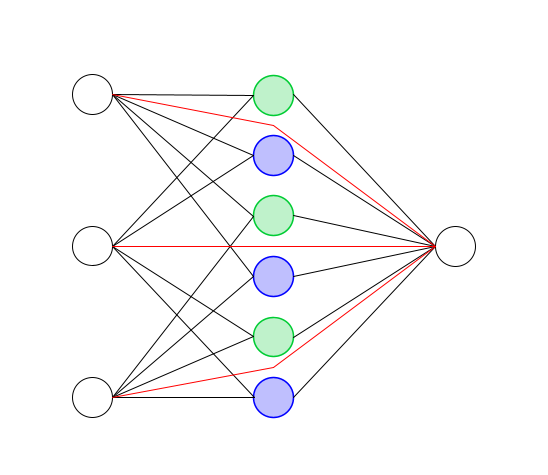
\includegraphics[height=\moyen]{pict/chnet1}
	\caption{Architecture d'un réseau de choquet}
	\label{fig:chnet1}
    \vspace{-10pt}
    \begin{center}
        \tiny
        \textit{
        En bleu, des neurone appliquant pour fonction principale $\min(X)$. \\
        En vert, des neurone appliquant pour fonction principale $\max(X)$.
        }
    \end{center}
\end{figure}
\vspace{-12pt}
On peut voir que trois problemes non triviaux se posent (\textit{cf.}\ \ref{subsec:réseau-de-neurones}) :
\begin{itemize}
    \item Les neurones collorées n'appliquent pas une simple application linéaire.
    \item Les neurones ne sont pas reliés en mode Dense mais en convolution.
    \item Certains neurones passent des informations en sautant une couche de neurones.
\end{itemize}


\paragraph{Une autre piste à alors été envisagée :}
Créer un réseau simple comme dans la figure\ \ref{fig:net3}.
Dans ce réseau, aucuns neurone n'a de fonction complexe :
ceux de gauche sont les entrées et
celui de droite fait le produit scalaire avec un vecteur poids.
\begin{figure}[H]
    \center
    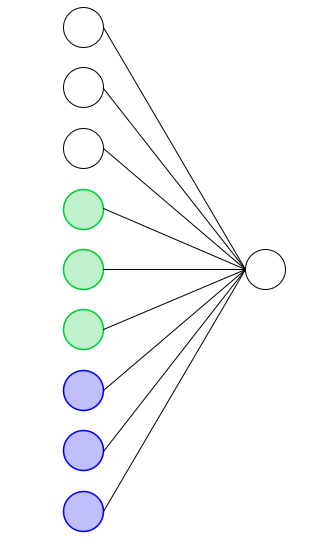
\includegraphics[height=\petit]{pict/net3.png}
	\caption{Réseau alternatif}
	\label{fig:net3}
\end{figure}
\vspace{-12pt}
Ce réseau est bien plus simple à générer : c'est un réseau \emph{Dense} de taille $9$ en entrée.
Et plus généralement $n^2$ pour un vecteur de taille $n$.


\rbox{Démonstation :}
{
Prenons un vecteur de taille $n$,
Le but est d'énumerer le nombre de neurones utiles a l'équation\ (\ref{eq:choquet}).
Le resultat est le suivant :
\begin{equation}
    n + \dbinom{n}{2} + \dbinom{n}{2} = n + 2 \times \frac{n(n-1)}{2} = n^2
\end{equation}
}

Il faut alors créer un vecteur d'entrée à partir une base de donnée d'aprentissage.
Cela se fait simplement en concaténant le vecteur $X$ avec les elements pris deux à deux passés
dans les fonctions min et max.\\


Lors de la descente de gradient, le réseau traite les poids indiférement,
pour les récupérer les poids de l'équation\ (\ref{eq:choquet})
il sufit de prendre les $n$ premiers pour $W$,
les $\frac{n(n-1)}{2}$ suivant pour $W_m$
et les $\frac{n(n-1)}{2}$ derniers pour $W_M$.
